\documentclass{article}

\usepackage{graphicx}
\usepackage{tikz}
\usepackage{tikzsymbols}
\usetikzlibrary{calc,patterns,shapes.geometric}
\pagestyle{empty}
\usepackage[margin=0pt]{geometry}
\geometry{papersize={14in,12in}}

\def\centerarc[#1](#2)(#3:#4:#5){\draw[#1] ($(#2)+({#5*cos(#3)},{#5*sin(#3)})$) arc (#3:#4:#5);}

\begin{document}
	\begin{figure}
		\centering
		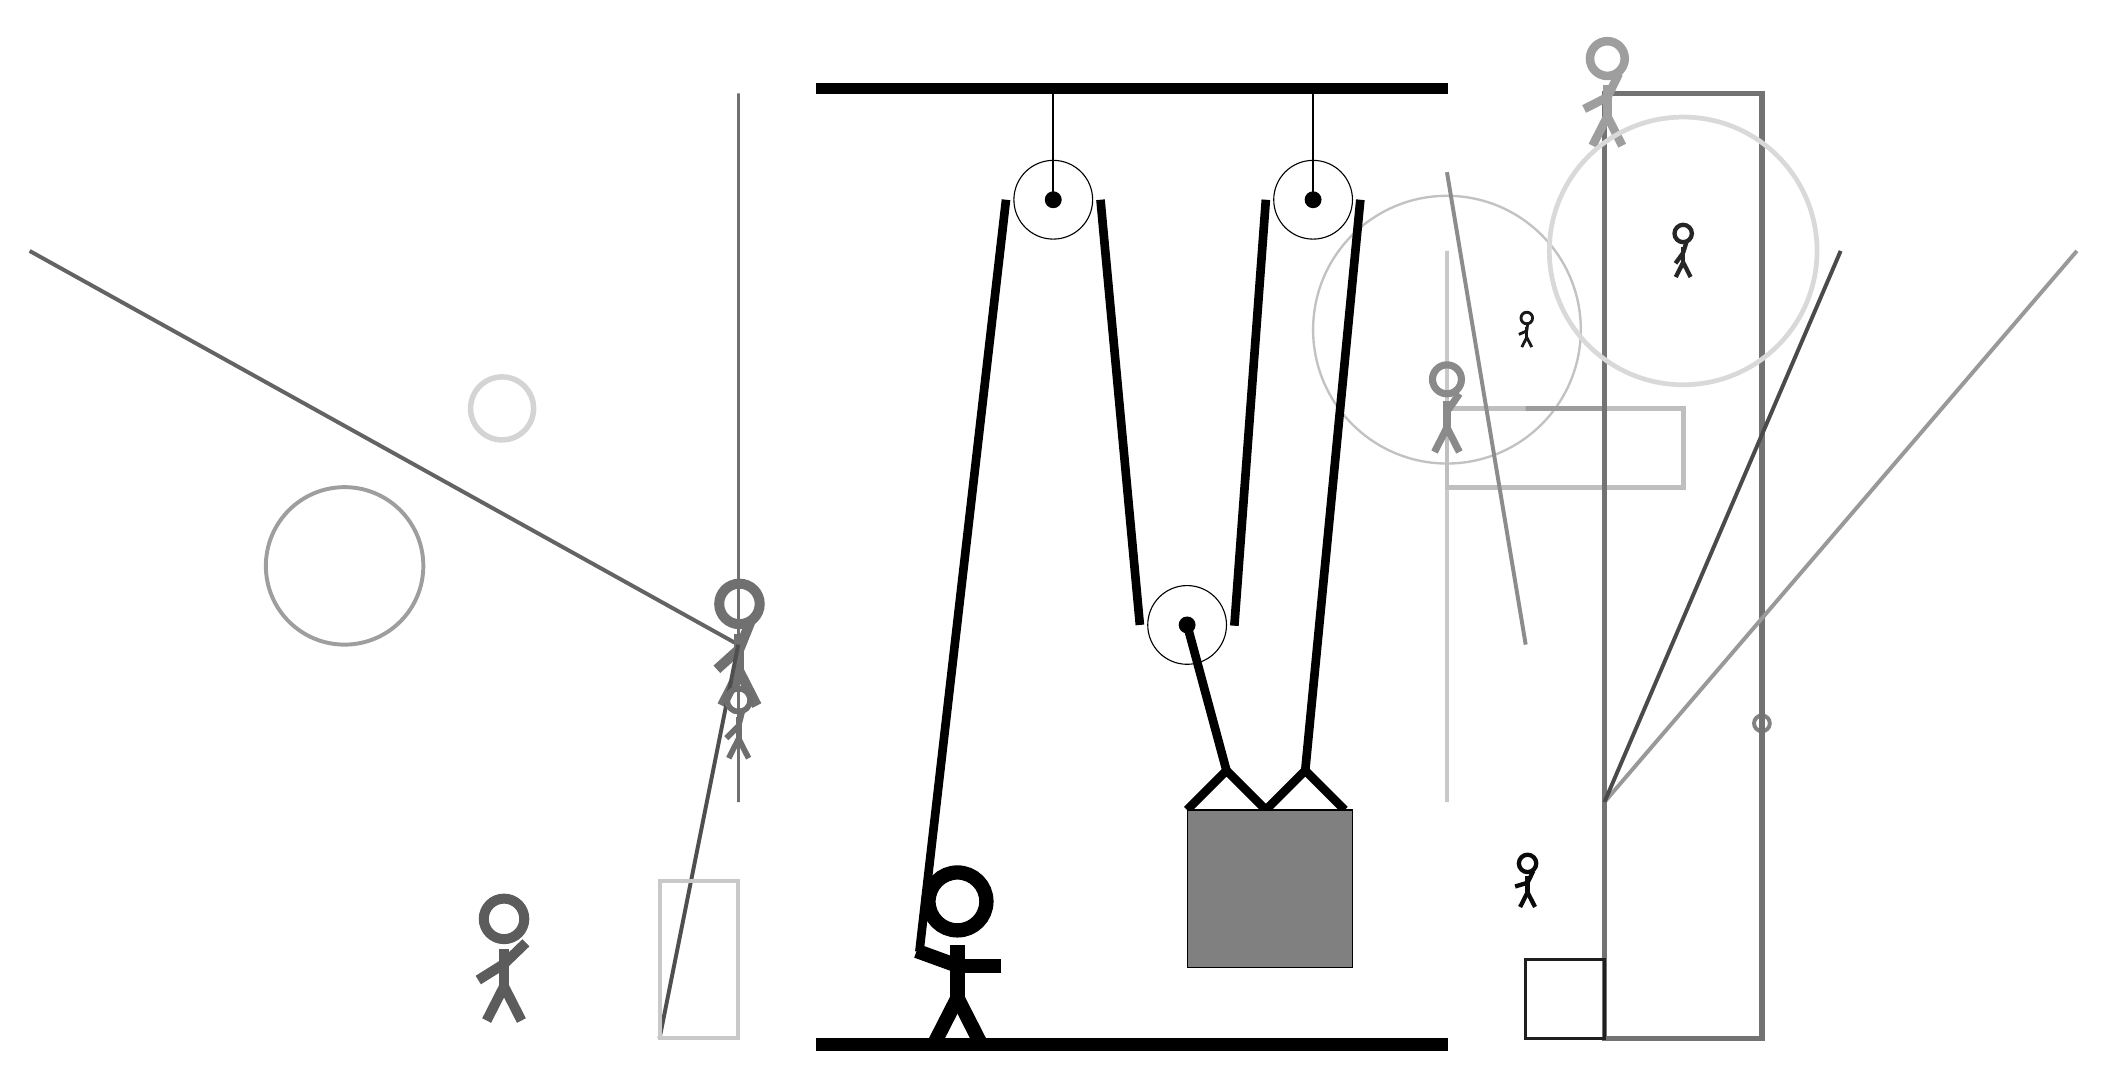
\begin{tikzpicture}
			%%%%% START %%%%%
			
			\draw[fill=black] (-2, 9) rectangle (6, 9.125);
			
			\draw (1, 7.65) circle (0.5);
			\draw[fill=black] (1, 7.65) circle (0.1);
			\draw[thick] (1, 7.65) -- (1, 9);
			
			\draw (4.3, 7.65) circle (0.5);
			\draw[fill=black] (4.3, 7.65) circle (0.1);
			\draw[thick] (4.3, 7.65) -- (4.3, 9);
			
			\draw [line width=0.3mm, color=black!24](6, 6) circle (1.7);
			
			\node[line width=0.7mm, color=black!90] at (7, 6) {\Strichmaxerl[2][24][83]};
			\node[line width=0.3mm, color=black!64] at (-6, -2) {\Strichmaxerl[7][32][44]};
			\node[line width=0.7mm, color=black!85] at (9, 7) {\Strichmaxerl[3][54][73]};
			\draw[line width=0.5mm, color=black!21] (6, 0) rectangle (6, 7);
			\draw [line width=0.5mm, color=black!38](-8, 3) circle (1.0);
			\draw[line width=0.5mm, color=black!61](-3, 2) -- (-12, 7);
			\draw[line width=0.4mm, color=black!26] (8, -2) rectangle (8, 8);
			\draw [line width=0.7mm, color=black!17](-6, 5) circle (0.4);
			\draw[line width=0.4mm, color=black!56] (-3, 9) rectangle (-3, 0);
			\draw[line width=0.6mm, color=black!25] (6, 4) rectangle (9, 5);
			\node[line width=0.3mm, color=black!56] at (-3, 2) {\Strichmaxerl[7][42][68]};
			\draw[line width=0.7mm, color=black!39] (8, 5) rectangle (7, 5);
			
			\draw[line width=0.5mm, color=black!69](-4, -3) -- (-3, 2);
			\draw [line width=0.5mm, color=black!49](10, 1) circle (0.1);
			\draw[line width=0.7mm, color=black!55] (8, 9) rectangle (10, -3);
			
			\node[line width=0.4mm, color=black!46] at (6, 5) {\Strichmaxerl[5][89][55]};
			\draw[line width=0.5mm, color=black!21] (-3, -3) rectangle (-4, -1);
			\draw[line width=0.5mm, color=black!40](8, 0) -- (14, 7);
			\node[line width=0.5mm, color=black!96] at (7, -1) {\Strichmaxerl[3][17][64]};
			\node[line width=0.5mm, color=black!38] at (8, 9) {\Strichmaxerl[6][27][64]};
			\node[line width=0.5mm, color=black!57] at (-3, 1) {\Strichmaxerl[4][45][76]};
			\draw [line width=0.6mm, color=black!15](9, 7) circle (1.7);
			\draw[line width=0.5mm, color=black!71](8, 0) -- (11, 7);
			\draw[line width=0.5mm, color=black!45](7, 2) -- (6, 8);
			
			\draw [line width=0.6mm, color=black!34](8, 2) circle (0.0);
			\draw[line width=0.4mm, color=black!88] (8, -2) rectangle (7, -3);
			
			\draw (2.7, 2.25) circle (0.5);
			\draw[fill=black] (2.7, 2.25) circle (0.1);
			
			\draw[line width=1.1mm]  (2.7, -0.1) -- (3.2, 0.4) -- (3.7, -0.1) -- (4.2, 0.4) -- (4.7, -0.1);
			\draw[fill=black!50] (2.7, -0.1) rectangle (4.8, -2.1);
			
			\draw[line width=1.1mm](-0.7, -1.9) -- (0.4, 7.65);
			\centerarc[line width=1.1mm](1, 7.65)(0:180:0.6);
			\draw[line width=1.1mm](1.6, 7.65) -- (2.1, 2.25);
			\centerarc[line width=1.1mm](2.7, 2.25)(180:370:0.6);
			\draw[line width=1.1mm] (3.3, 2.24) -- (3.7, 7.65);
			\centerarc[line width=1.1mm](4.3, 7.65)(0:180:0.6);
			\draw[line width=1.1mm](4.2, 0.4) -- (4.9, 7.65);
			\draw[line width=1.1mm] (3.2, 0.4) -- (2.7, 2.25);
			
			\node at (-0.2, -2) {\Strichmaxerl[10][-20][0]};
			
			\draw[fill=black] (-2, -3) rectangle (6, -3.15);
			
			%%%%% END %%%%%
		\end{tikzpicture}
	\end{figure}	
\end{document}